\chapter{Team assignments}

In this chapter, we are describing motivation, development, support and usage of team assignments. We decided to introduce this concept into educatioal process during the spring of 2015 on some courses, such as Modern Approaches to Webdesign or Algorithms and Data Structures. We finished specifications during summer of 2015 and by start of the winter semester   Courses 2 Assignments module was reimplemented to support this change. After that time, this module was ready but we continued to support it's further development to met all of the students needs.

This work is also a subject of other researchers at our faculty such as Veronika Dropcova's research \cite{dropcova}. In this work, we focus on semantics and implementations whereas other researchers are focusing on pedagogical aspects of this work.


\section{Motivation}

Computer Science students are often taught many different types of algorithms, matematics and programmings languages. This is very beneficial to them since many hard skills will be reqired in their future career. But on the other side of this, these students are lackings skills in teamwork, constructive critisism, the ability of self\-reflection or job evaluation.  These skills are essential in ther future jobs or science career but still none or very little effort is put to teach students these skills. 

This is why we are introducing new concepts of assignments for students.  In this chapter, we focuse on implementing and usage of one of these concepts, team assignments with peer and team review. With usage of this term, we mean an assignment, which students solve in small teams, submit their solutions and then review other teams work and their teammates. Each part of this teaching process is designed to teach them specific soft skills. Working in teams teaches students communication, leadership and teamwork. Filling out team reviews is teaching self\-reflection whereas reviewing other team's work is developing the ability of constructive critisism. Each of this mentioned concept is described in detail in following subsections.


\section{Semantics and implementation}
Now, we we move to semantics and implementation of team assignments in Courses 2 Learning Management System. It was very challenging to alter the database model and source code while still persisting old functionality without any bugs. Results presented in this section are result of extensive development, refactoring and testing because old design of Assignment module did not expect to provide an inteface, where one submission could be linked with whole team (multiple students). We also had to build this system as secure as possible not to allow students to alter any unwanted data. This process of testing and bugfixing took us few months.

\subsection{Representation}

\subsubsection{Database}
Final representation of teams in database is shown on Figure \ref{assignmentdatabase} in Appendix A. On this figure, elements added in this work are marked red, original elements are black. We decided to represent basic team with two tables \texttt{assignment\_team} and \texttt{assignment\_team\_member}.

The first one is used only for pairing the team with specific assignment and retrieving its name. Elements represented by this table are checked for duplicity so there can not be two teams with the same name in one assignment.

The second one serves for remembering which student is in which team. This table is also used for student invites (column \texttt{accepted} which we explain later. There is also a redundant attribute \texttt{assignment\_id}, which could be retrieved from the first table but adding this redundancy helps reduce database load and database query simplicity.

There are also tables \texttt{assignment\_round\_team\_question}, \texttt{assignment\_round\_team\_answer} and \texttt{assignment\_rount\_team\_rating} that plays part in team reviewing which is to be explained in Section \ref{sec:teamreview}.

We also had to alter old database table of \texttt{assignment} and \texttt{assignment\_round} and add columns to specify team creation, limits, deadlines and reviews. These names are hovewer self\-explanatory.

\subsubsection{Models}
For managing teams, we created \texttt{Assignment\_team\_model} located in \\ \texttt{application/modules/assignments/models/} directory. This model offers a handful of methods for creating, updating, deleting and managing teams.

\begin{lstlisting}[caption={Method for accepting team invites},label={lst:teaminvite}]
public function accept_invite($invite_id, $user_id)
{
    $where = array (
        'id'      => $invite_id,
        'user_id'        => $user_id,
    );

    $input = array(
        'accepted'       => '1',
    );

    $result = $this->db->where($where)->update('assignment_team_member', $input);
    return $result;
}
\end{lstlisting}

On Listing \ref{lst:teaminvite} we can see method for accepting team invites in team model (these will be explained later). As we minimal database model with a little redundancy, these methods can be kept very simple.

For managing team reviews, we created \texttt{Team\_reviews\_model}. This model is used both for administration and submissions of peer reviews. We will explain team reviews in Section \ref{sec:teamreview}.

We also had to refactor \texttt{Assignments\_model} and \texttt{Admin\_model} as they could not work with the team data. These refactorings often changed behaviours of these models because the original version of module did not expected to be extended this way. We will provide an example in Subsection \ref{sec:peerreview} when speaking of peer review. This was among most impacted and problematic parts as it was deeply wired into whole system and any changes could cause a lot of bugs.

\subsubsection{Controllers}
Controllers for team projects are split into two categories. \texttt{User} and \texttt{Admin} category.

User controllers are located in \\ \texttt{application/modules/assignment/controllers/user} folder and are used only for user actions. For purposes of this work, we had to refactor \texttt{Assignment} controller which previously managed only submitting of submission. Now its functionality is extended and this controller is also used for managing team changes (create, invite, accept invite, leave team). Then, we added \texttt{Team\_Review} controller which serves as the manager for team reviews.

Admin controllers are located in \\ \texttt{application/modules/assignment/controllers/admin} folder and also had to be refactored extensively. We created \texttt{Manage\_team\_reviews} controller which serves as manager of team reviews. There was already done controller for managing peer reviews called \texttt{Manage\_reviews} about which we will explain later. It is also worth mentioning \texttt{Assignments} controller which serves as managing class for assignments (creating, editing, evaluating) and also for team management (create, edit, edit members)

\subsubsection{Views}
Finally, views of team assignments can be found in \\ \texttt{application/modules/assignment/views} directory. These are also divided into two groups user and admin part, each with corresponding folder. For our purposes, we created a many more new views but these are relatively easy to understand.

\subsection{Team assignment creation}
We will now go through team assignment flow, as we designed it. During this, we will explain also the problems we encountered and some solutions.

The teacher can create a team assignment in teacher's assignment administration interface. This interface is the same as for creating a normal assignment. The only difference is that teacher must allow the assignment to be team assignment, set deadlines for team forming and fill, how many students he expects to be in each team. The teacher can set lowest and highest number of students in each group without any limitations. This settings are then stored in \texttt{assignment} database table under values \texttt{is\_team}, \texttt{team\_min\_members}, \texttt{team\_max\_members}, \texttt{team\_forming\_closes}.

\subsection{Team forming}
After the start time of team forming has passed and before team forming deadlines, students are required to create or join a team. This is implemented as shown on Figure \ref{team_forming}. Leader of the team can enter team name, which has to be unique for the course. After he created the team, he automatically joins this team and is reqired to invite his classmates to join. There is a limitation of how many students can be invited, based on maximum number of students in one team. This means that he can only invite as many friends as is the maximum number allowed by the teacher. He can, however, delete this invites and invite a different classmate. Also, any member of the team can invite another student of the course.

\begin{figure}[h]
    \centering
    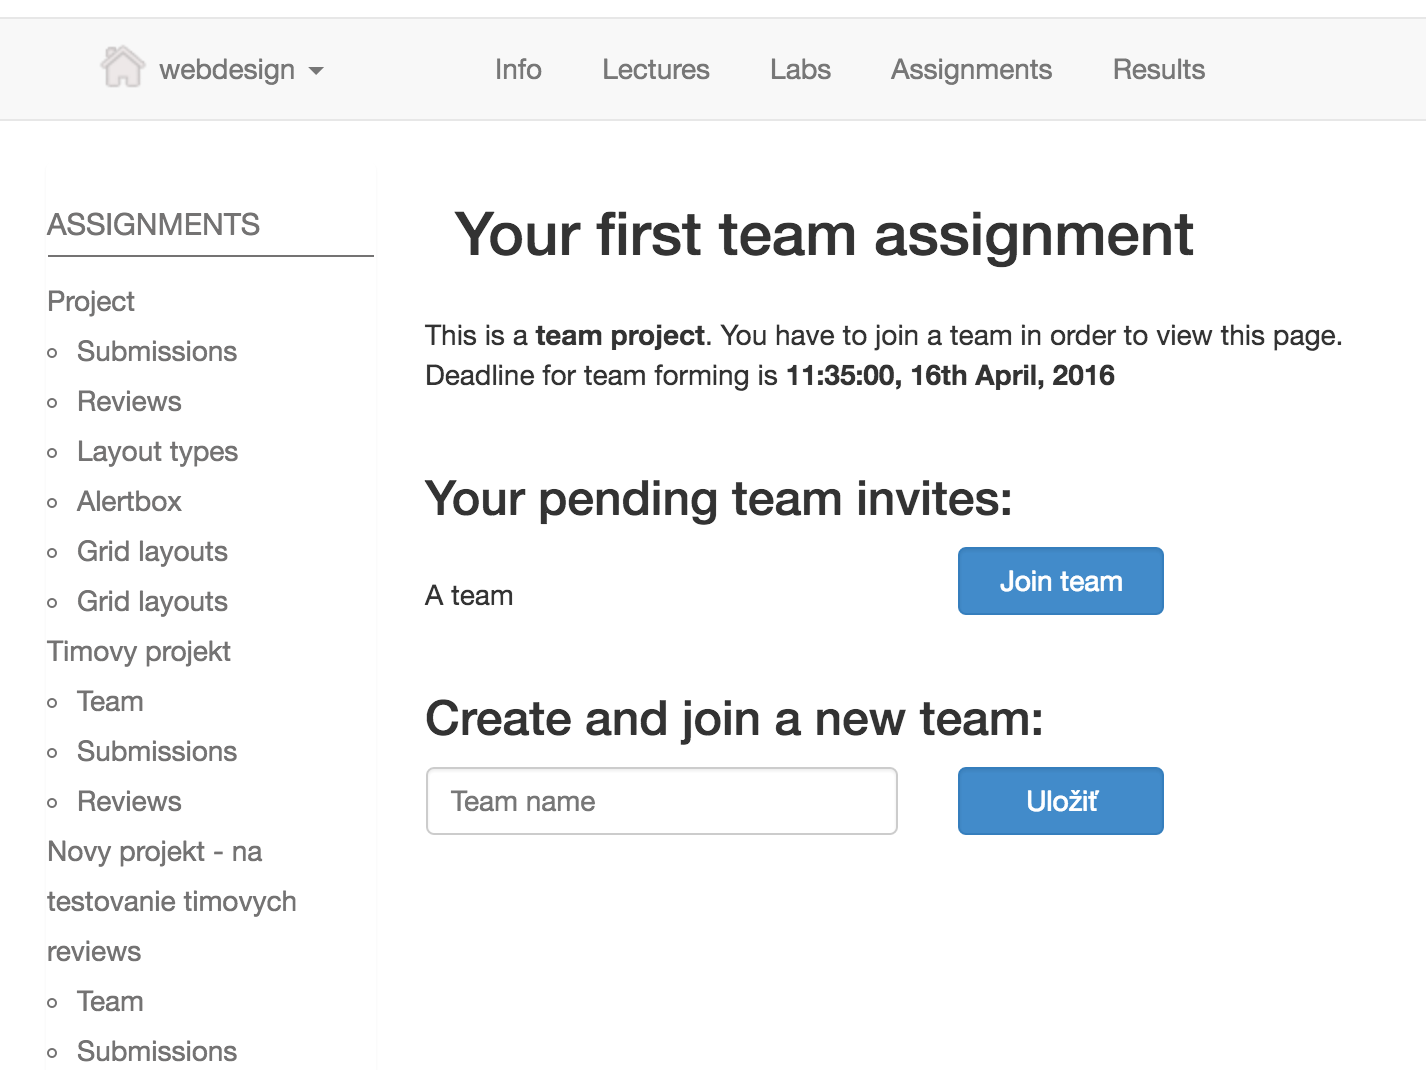
\includegraphics[width=\textwidth]{images/teamforming.png}
    \caption{Team forming}
    \label{team_forming}
\end{figure}

If the student accepts an invite, all his other invites are made invalid so these teams can invite different students. This student can also leave the team if he wants, but the team has to invite him again if they want him to join again. There is also no option to kick another team member from team, he can only leave willingly. If all members of the team left, the team is deleted and dismissed.

Another thing to mention, while the team does not have enough members specified by the teacher, there is a notification shown to each member. This is done to ensure that the team does not forget about this.

After the team forming deadline, no student can join, create nor leave the team. After this deadline, only teacher can edit team members and still create new team. 

\begin{figure}[h]
    \centering
    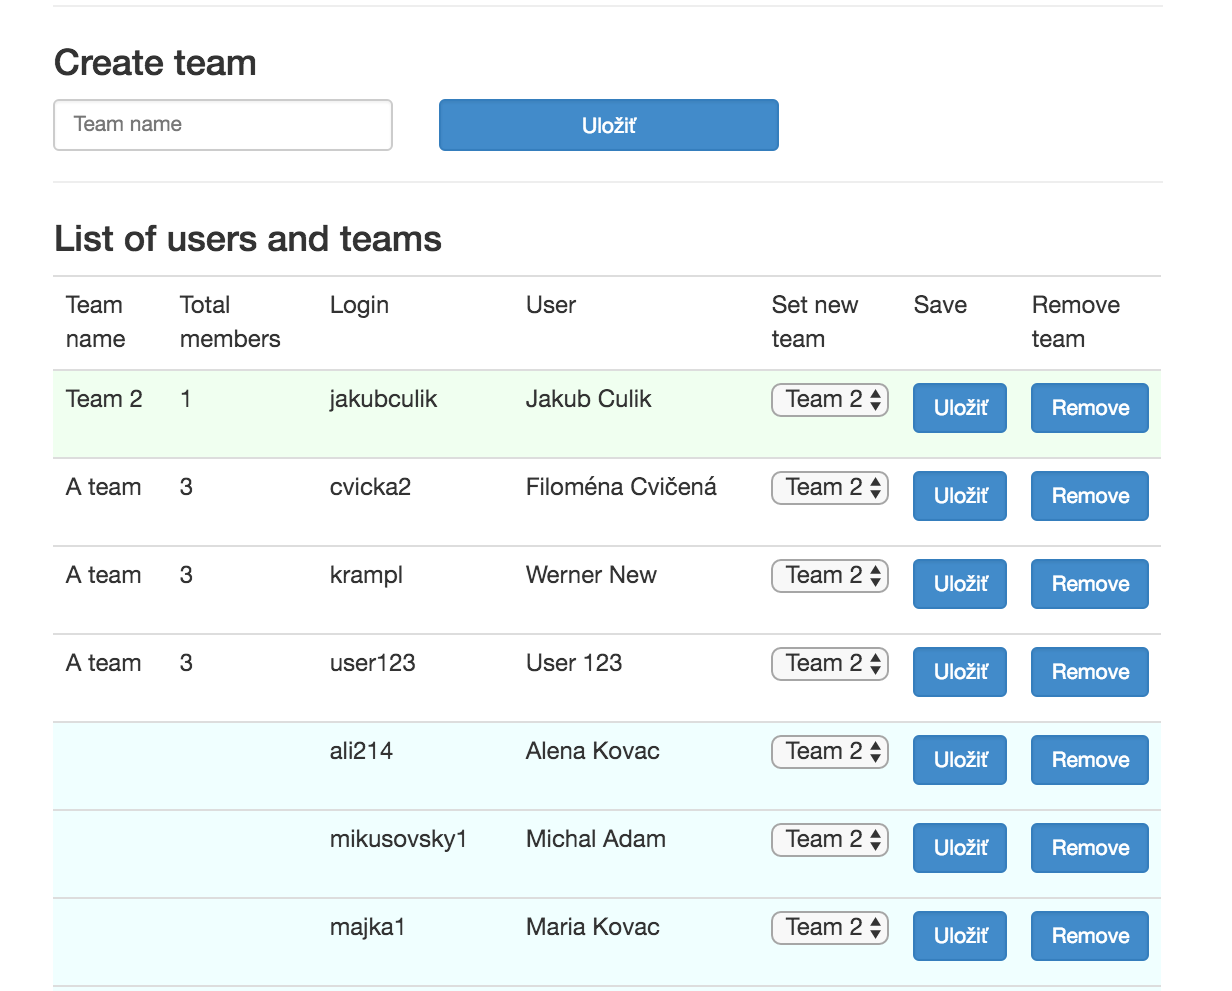
\includegraphics[width=\textwidth]{images/teamadmin.png}
    \caption{Team administration}
    \label{team_forming}
\end{figure}

The teacher can in administration see the list of the teams as shown on Figure \ref{team_forming}. During the development, we tried multiple types of interfaces and this is the one that was selected. This interface offers simple access to each student and team forming or editing.


\subsection{Assignment submission}
In the next step, after all of the teams are formed, and assignments are open students can submit their assignment solutions. Since we are speaking about team projects, it is enough if only one of the team members submit this submission provided that all of the members participated on it. So if one students submits the solution, all members of the team should see it and be rated for it.

This could be done by multiple ways. As we see on Figure \ref{assignmentdatabase} one submission is represented by a \texttt{assignment\_submission} table. For pairing submission with users were used parameters \texttt{user\_id} and \texttt{submission\_id}. So for team projects, we could just create a new table like \texttt{assignment\_team\_submission} with parameter \texttt{team\_id} instead of \texttt{user\_id}.

This approach would however be very inefficient and would led to code duplicity and refactoring. Instead of this, we chose to fix this problem in model layer of Assignment module. All submissions for a team member can be retrieved by joining the tables  \texttt{assignment}, \texttt{assignment\_team} and \texttt{assignment\_team\_member}. Some people could argue that joining three database tables may lead to inefficiency but it is not true. We do not expect to have millions of teams and students in our database so we could prioritize code simplicity and reusability instead of effectivity on large datasets.

\subsection{Peer review}
\label{sec:peerreview}
Peer review is another important part of team projects. By this term we mean reviewing work of other teams. Each team gets 3 other submissions to review. Reviewing process includes understaning of this solution, answering questions defined by a Teacher and submitting them. We also decided that we will for now accept reviews from one user for whole team. So it is enough if the team choses one member, who will submit team reviews. This was decided also for research purposes by Veronika Dropcovas research \cite{dropcova}. 

Team review deadlines are set by the teacher in assignment administration and then stored in \texttt{assignment\_round} table. We designed these reviews not to be assigned automaticaly after the reviewing period began but an action from the teacher is required. The teacher must press the button for peer review assignment in administration. The reason for this is that sometimes a student forgets about deadline or tries to submit a submission few minutes after deadline. In such case, if peer reviews were assigned automatically after the submitting period ended, this students work would not be evaluated by other students.

In peer reviews we were able to use original algorithm by Jakub Culik \cite{culik} with minor changes. This could be done by clever choice of data model, which can act as an individual, not team project. As we said in previous subsection, teams are not directly connected to submissions in data model but users are. With this hack, we could put data to review assigning algorithm which outputs which users has to review which submissions.

Information about which submissions has the user review therefore cannot be seen on database layer. But we can also cleverly merge the team tables in model layer and retrieve the needed information.

\begin{lstlisting}[caption={Retrieving information about peer reviews},label={lst:peerreviewlisting}]
public function get_to_review($assignment_id)
{
    $where = array(
        'a.assignment_id' => $assignment_id,
        'a.course_id'     => $this->cid,
    );

    $team = $this->get_team_members($this->uid, $assignment_id);

    return $this->db->select('a.*, b.submission, u.user_name, r.submission_type, r.name as round_name, r.reviewing_opens, r.reviewing_closes, r.visibility, q.name as assignment, assign.is_team as is_team, t.name as team_name')
        ->from('assignment_rating_batch a')
        ->join('assignment_submission b', 'a.submission_id = b.id')
        ->join('assignment_round r', 'a.round_id = r.id')
        ->join('assignment q', 'a.assignment_id = q.id')
        ->join('user u', 'b.user_id = u.id')
        ->join('assignment assign', 'assign.id = a.assignment_id')
        ->join('assignment_team_member atm', 'atm.assignment_id = a.assignment_id AND atm.user_id = b.user_id AND atm.accepted = 1', 'left')
        ->join('assignment_team t', 't.id = atm.team_id', 'left')
        ->where($where)
        ->where_in('a.user_id', $team)
        ->get()
        ->result_array();
}
\end{lstlisting}

As on Listing \ref{lst:peerreviewlisting}, for retrieving information about peer reviews, we must join the team tables. This solution offers great code reusability but there's a price to pay in joining multiple tables. This tables are hovewer kept reasonably small and SQL optimizer in any database system can easily optimize this query.

This solution is the best also for different reasons. When we need to retrieve all submitted reviews for any team member, it might happen that each review is filled and submitted by different member. We must however display all of them. Merging tables and querying for all team members is therefore superior option to duplicating the database and creating many tables.  

\subsection{Teamwork review}
\label{sec:teamreview}
Teamwork is filled by each team member and usually consists of two parts which are predefined by the teacher. 

The first part looks similar to peer reviewing. Student has to answer multiple questions about each team member. These questions usually asks information about how much work each member has done, how he did it and may be asking for feedback for this user. Each team members is then shown what other team members responded about him anonymously. This is providing him feedback about what skills or behaviours should he improve.

The second part is called teamwork rating consists of team evaluation. The student has to split 100 points between all other members. For example, if there are three other team members, the student can give 30, 30 and 40 points to his teammates. These points are then summed up and play role in final evaluation for evaluated student. 

We also had to come up with an algorithm to generate these points for users who refused to participate in teamwork review. At first, we tried to implement some sophisticated generation based on other students answers but this approach did not work well. At the end we chose the simplest solution and divide this points equally between all students. The reason for this was that even though it was easy to find and implement some statistic based solution, this solution might not be objective in some cases. For example only one or two students answered, their percentage could be very subjective and a good student could get not too many points.


\begin{figure}[h]
    \centering
    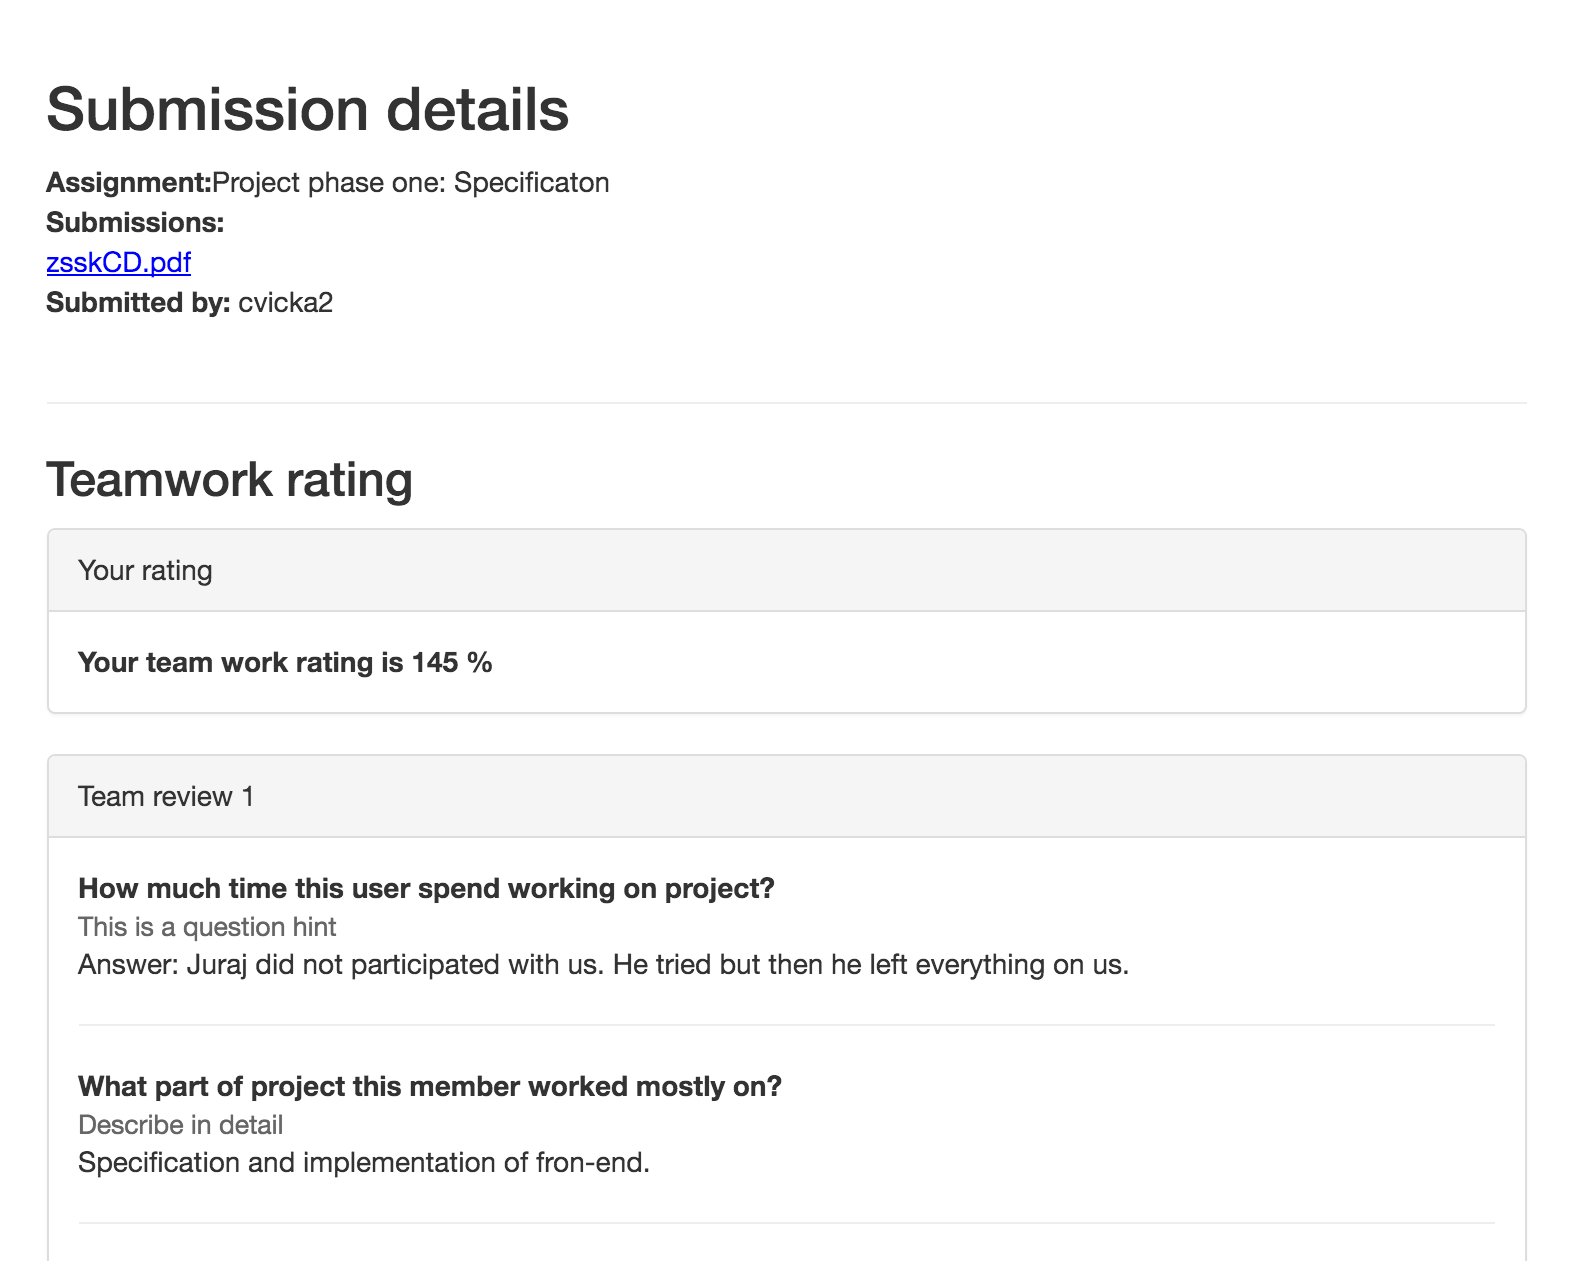
\includegraphics[width=\textwidth]{images/teamreview.png}
    \caption{Team reviewing results}
    \label{team_reviewing}
\end{figure}

Results of teamwork reviewing are shown on Figure \ref{team_reviewing}. This screenshot is taken from the assignment submission page. At first, we decided to show submission details and enabled students to download their submission.

In the next section we show teamwork rating as a sum of all individual teamwork ratings of this team member for this project round. 

The last part are all of submitted teamwork reviews written by individual team members. These reviews are groupped by team members and ordered by order of questions defined by the teacher.


\subsection{Teacher's evaluation}
The last part of team projects is teacher's evaluation. This evaluation takes place in assignments interface.

\begin{figure}[h]
    \centering
    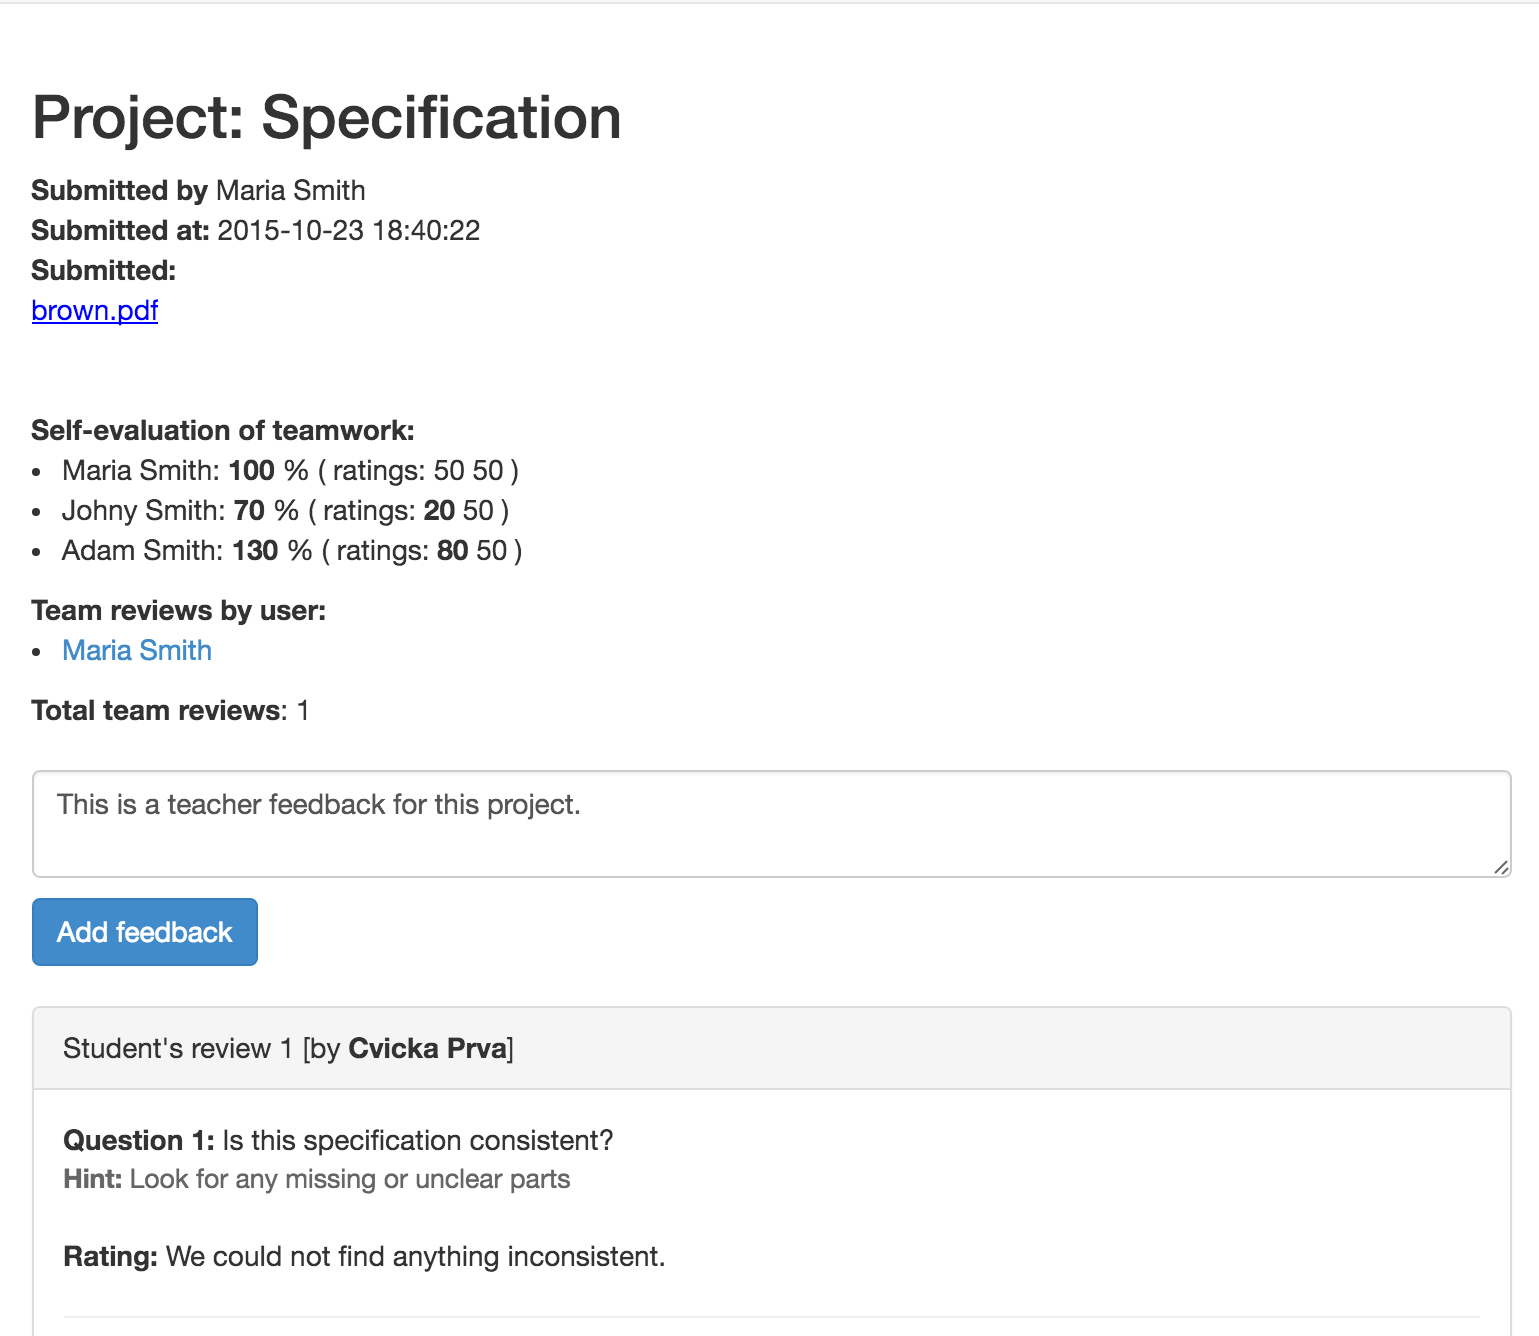
\includegraphics[width=\textwidth]{images/teamprojectevaluation.png}
    \caption{Team project evaluation}
    \label{team_submission_admin}
\end{figure}

First part of teacher's is build to show all of the submissions ordered by team name. There are also some more information, like submission date, assigned reviews and evaluation present. The teacher is then supposed to open an assignment submission page, as show on Figure \ref{team_submission_admin}.

Second part of teacher's evaluation is shown on Figure \ref{team_submission_admin}. This is a team project, but name of the student who submitted this submission is shown on the top of the page. This can be done easily with our database design. 

The teacher is then supposed to review the team's submission and evaluate it. 

In the next step, there are shown results of team evaluation for each memeber of the team. In each row, the fist number is the total percentage received. Then, the bold numbers are results of evaluation of each team member. If some team member did not submit his team evaluation, we automatically divide his points to other team members. These auto generated numbers are not bold.

These information are shown mostly for evaluation purposes, because the teacher can divide the evaluated points for project among the best team members. He can also award the best members of the team with bonus points.

As we see on Figure \ref{team_submission_admin}, only one team evaluation is submitted. Results for the other two team members are auto generated.

The next section of evaluation offers a teacher links to team reviews by users. These information had to be generated on different page for clarity purposes. It would be to much noise if they were shown together with other types of reviewing.

Also, the number of total submitted team reviews is avaible for a teacher.

Then, there is a feedback form, which serves as a feedback shown on student's submission page.

And finally, on the bottom of the page we show results of peer reviews. These reviews are groupped by submitted users and ordered by order of questions defined by a teacher.

Final results of the evaluations has to be, because of Courses 2 box modularity, put into different module of Courses 2, called Results Module. We see this inefficient for the teacher and also for students so there is still a space for future improvements.

\section{Conclusion}
TODO: Should I write a conclusion for this chapter?
